\documentclass[conference]{IEEEtran}

\usepackage{graphicx}
\usepackage{xcolor}
\usepackage{hyperref}
\usepackage{booktabs}
\usepackage{listings}
\usepackage{cite}
\usepackage{tikz}
\usetikzlibrary{positioning,arrows.meta,fit}

\definecolor{todocolor}{RGB}{192,0,0}
% Use \todoblock{label}{instructions} to mark a section that still needs
% real data from your own Wireshark captures. Search for "todoblock" and
% delete every occurrence before final submission.
\newcommand{\todoblock}[2]{%
  \par\noindent\textbf{\textcolor{todocolor}{[#1]}}~\textit{\textcolor{todocolor}{#2}}\par%
}

\lstset{
  basicstyle=\ttfamily\footnotesize,
  breaklines=true,
  columns=flexible,
  frame=single,
  framerule=0.3pt,
}

\begin{document}

\title{
  
\includegraphics[height=1.05cm]{figures/hsrw_logo.png}
  \hfill
  
\includegraphics[height=1.05cm]{figures/crl_logo.png}\\[10pt]
  Multi-Protocol Traffic Generation and Analysis:\\
  A Containerized System for HTTP/2, QUIC, MQTT and Raw TCP/UDP
}

\author{
  \IEEEauthorblockN{Amine Ahamri}
  \IEEEauthorblockA{
    Mobile \& Internet Computing\\
    Hochschule Rhein-Waal\\
  }
}

\maketitle

\begin{abstract}
This report describes a containerized system for generating and controlling
network traffic. It covers five protocols at once: HTTP/2, QUIC, MQTT, TCP and
UDP. 15 Docker containers make up the system. A central controller reads
YAML traffic profiles and drives four generators through a REST API. The
system supports four sending patterns: constant, periodic burst, linear ramp,
and Poisson-distributed random intervals. It also runs an autonomous Adaptive
Control loop that reacts to error rates and latency, plus a stealth mode for
the TCP/UDP generator that hides its statistical fingerprint. This report
covers the architecture, the implementation decisions behind it, the
configuration format, and the Wireshark-based traffic analysis.
\end{abstract}

\begin{IEEEkeywords}
HTTP/2, QUIC, MQTT, Docker, traffic generation, Wireshark, behavioral fingerprinting, adaptive control
\end{IEEEkeywords}

\section{Introduction}

A normal office network never carries just one protocol. At any moment there is
web traffic, IoT sensor data, video calls and background sync jobs all sharing
the same wire. Studying how these protocols behave together, how they fail, and
how easy they are to tell apart from the outside, needs a testbed that can
actually produce that mix on demand and let you turn the dials while it runs.

This project builds exactly that testbed, based on the assignment in
\cite{hsrwassignment}. It generates traffic for five protocols at the same
time: HTTP/2 \cite{rfc7540}, QUIC/HTTP-3 \cite{rfc9000, rfc9114}, MQTT
\cite{mqtt5} with all three QoS levels, and raw TCP and UDP. Everything runs
as 15 Docker containers orchestrated with Docker Compose \cite{dockercompose},
started with one \texttt{docker-compose up}. A central controller loads a YAML profile
and tells four traffic generators what to send and how fast; a web dashboard
lets you change any of that live, without restarting anything.

Beyond the basic rate and payload-size knobs, the system implements four
sending patterns (constant, periodic burst, linear ramp and Poisson-distributed
random intervals), a stealth mode that makes the raw TCP/UDP generator
statistically indistinguishable from normal traffic, and an autonomous Adaptive
Control loop that scales a generator's rate up or down based on the error rate
it is currently seeing, with no human in the loop.

The rest of this report is organized as follows. Section II describes the
architecture. Section III walks through the implementation decisions that
mattered, and why they were made that way. Section IV documents the
configuration format. Sections V through VII present the Wireshark-based
traffic analysis, the failure-visibility results and the single- versus
multi-machine comparison. Section VIII reflects on what the data actually
showed about protocol behavior, and Section IX documents how AI tools were
used while building this.

\section{System Architecture}

The system has 15 containers on one Docker bridge network called
\texttt{mic-net}. Containers find each other by service name through Docker's
internal DNS, so \texttt{gen-http2} can simply call
\texttt{http://target-http2:8080} without anyone configuring an IP address
anywhere.

Ten of those containers carry the core pipeline described below; the
remaining five are the Mosquitto broker and four \texttt{tshark}-based
analyzer sidecars (one per target's network namespace), introduced at the
end of this section. The ten core containers fall into four groups. The \textbf{controller} (FastAPI,
port 8000) is the brain: it reads the YAML profile, drives the four generators
through their REST APIs, and runs the Adaptive Control loop. This loop is a
real feedback mechanism, not just a timer working through YAML phases. Every
few seconds the controller checks each generator's current error rate against
a threshold and, if it is crossed, scales that generator's rate down by a
bounded multiplier on its own, no human involved. Section III-E gives the full
description. The four \textbf{generators} (\texttt{gen-http2}, \texttt{gen-quic},
\texttt{gen-mqtt}, \texttt{gen-tcpudp}) each keep their own state and expose
the same four endpoints: start, stop, patch the config, get the status. They
are built on \texttt{httpx} (HTTP/2), \texttt{aioquic} \cite{aioquic} (QUIC),
\texttt{paho-mqtt} \cite{pahomqtt} (MQTT) and plain Python sockets (raw
TCP/UDP). The three \textbf{target services} (\texttt{target-http2},
\texttt{target-quic}, \texttt{target-tcpudp}) receive traffic alongside the
separately-counted Mosquitto broker \cite{mosquitto}. \texttt{target-http2} runs on Hypercorn
\cite{hypercorn}, the only ASGI server in the project that supports HTTP/2
natively. The \textbf{metrics collector} (Flask, port 9090) aggregates
everything into one \texttt{/metrics} response, and the \textbf{dashboard}
(a single static HTML file served over port 3000) polls the controller every
two seconds and renders the live state.

Reporting to the metrics collector is not symmetric across these
containers, and it is worth being precise about who reports and why. All four
generators post their own send-side counters (packets sent, error count,
current rate) to the collector, since the controller's Adaptive Control loop
reads those numbers. \texttt{target-http2} and \texttt{target-quic} also post
what they received, because both run custom code that can be instrumented
freely. Mosquitto cannot do this: it runs the stock
\texttt{eclipse-mosquitto:2} image with no custom instrumentation hook, so it
stays a black box. Every MQTT number in this report, throughput, latency,
QoS-level counts, comes only from \texttt{gen-mqtt} on the sending side, never
from the broker itself. \texttt{target-tcpudp} stays equally silent, but for
a different reason: it is meant to disappear cleanly when stopped, and the
resulting TCP RST is exactly what Section VI needs to see in a Wireshark
capture. A reporting connection on top of that would just be one more thing
that breaks when the container goes down, so it was left out on purpose.

Fig.~\ref{fig:architecture} shows how a request actually travels through the
system. The dashboard never talks to a generator directly; every change goes
through the controller, which is what makes it possible to log every
configuration change with a timestamp, as the assignment requires.

\begin{figure*}[t]
\centering
\resizebox{\textwidth}{!}{%
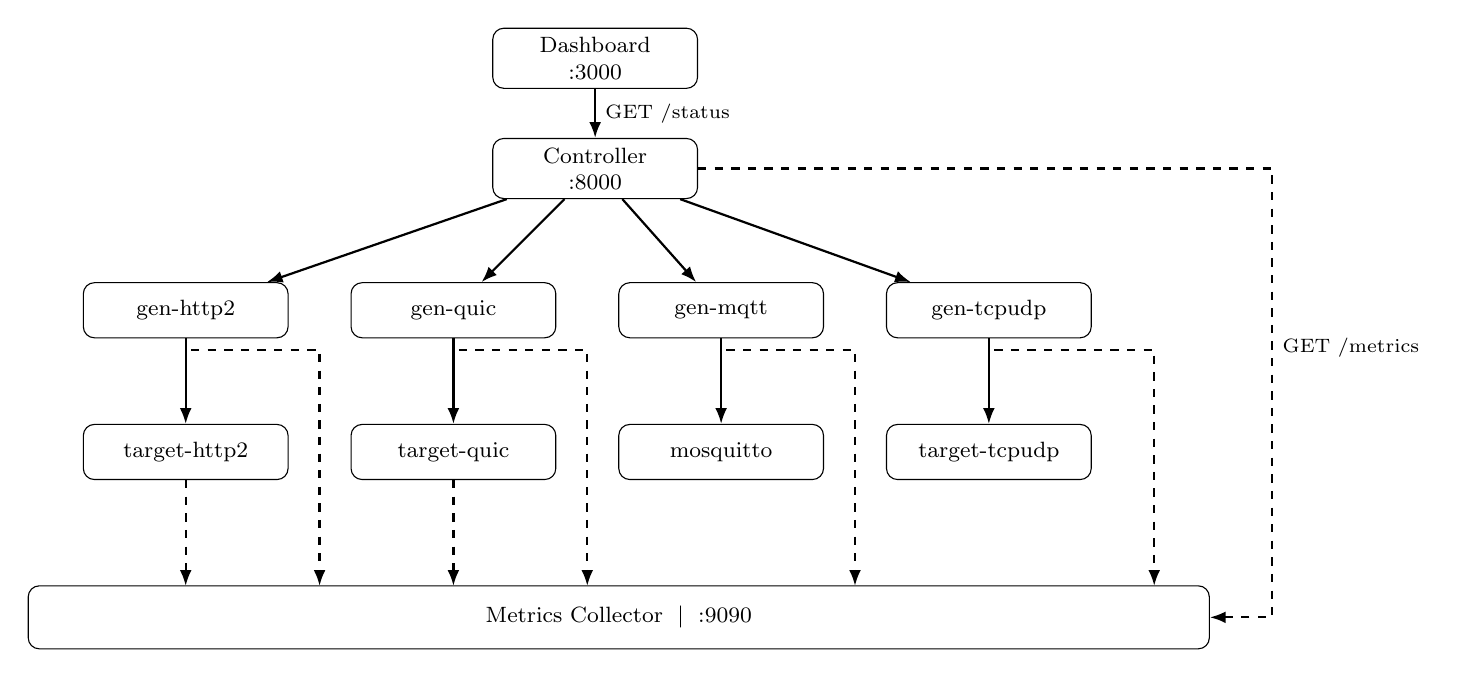
\begin{tikzpicture}[
  box/.style={draw, rounded corners, minimum width=2.6cm, minimum height=0.7cm, align=center, font=\footnotesize},
  arr/.style={-{Latex[length=2mm]}, thick},
]
\node[box] (dash) at (5.2,6.6) {Dashboard\\:3000};
\node[box] (ctrl) at (5.2,5.2) {Controller\\:8000};

\node[box] (h2)     at (0,3.4) {gen-http2};
\node[box] (quic)   at (3.4,3.4) {gen-quic};
\node[box] (mqtt)   at (6.8,3.4) {gen-mqtt};
\node[box] (tcpudp) at (10.2,3.4) {gen-tcpudp};

\node[box] (th2)    at (0,1.6) {target-http2};
\node[box] (tquic)  at (3.4,1.6) {target-quic};
\node[box] (broker) at (6.8,1.6) {mosquitto};
\node[box] (ttcp)   at (10.2,1.6) {target-tcpudp};

\node[box, minimum width=15cm, minimum height=0.8cm] (metrics) at (5.5,-0.5) {Metrics Collector \;\textbar\; :9090};

\draw[arr] (dash) -- (ctrl) node[midway, right, font=\scriptsize] {GET /status};
\draw[arr] (ctrl) -- (h2);
\draw[arr] (ctrl) -- (quic);
\draw[arr] (ctrl) -- (mqtt);
\draw[arr] (ctrl) -- (tcpudp);
\draw[arr] (h2) -- (th2);
\draw[arr] (quic) -- (tquic);
\draw[arr] (mqtt) -- (broker);
\draw[arr] (tcpudp) -- (ttcp);

\draw[arr, dashed] (th2) -- (0,-0.1);
\draw[arr, dashed] (tquic) -- (3.4,-0.1);

\draw[arr, dashed] (h2.south)     -- (0,2.9)  -- (1.7,2.9) -- (1.7,-0.1);
\draw[arr, dashed] (quic.south)   -- (3.4,2.9) -- (5.1,2.9) -- (5.1,-0.1);
\draw[arr, dashed] (mqtt.south)   -- (6.8,2.9) -- (8.5,2.9) -- (8.5,-0.1);
\draw[arr, dashed] (tcpudp.south) -- (10.2,2.9) -- (12.3,2.9) -- (12.3,-0.1);

\draw[arr, dashed] (ctrl.east) -- (13.8,5.2) -- (13.8,-0.5)
  node[pos=0.4, right, font=\scriptsize] {GET /metrics} -- (metrics.east);
\end{tikzpicture}%
}
\caption{Component diagram of the single-machine deployment. Solid arrows are
REST calls or raw protocol traffic. Dashed arrows show metrics reporting: all
four generators and the two custom-built targets post their counters up to
the collector; the long line on the right is the controller reading the
aggregate back out for the dashboard and for Adaptive Control. Mosquitto and
\texttt{target-tcpudp} have no dashed line on purpose, as explained in the
text.}
\label{fig:architecture}
\end{figure*}

The same decoupling that makes this diagram work on one machine is what makes
the two-machine deployment in Section VII possible without changing a single
line of code. Every generator already reaches its target through an
environment variable (\texttt{TARGET\_URL}, \texttt{TARGET\_HOST}, or
\texttt{BROKER\_HOST}), never through a hardcoded address. Splitting the
system across two hosts is therefore just a matter of pointing those
variables at a real IP instead of a Docker service name, as described in
Section VII; no overlay network or Swarm setup is needed for two machines on
the same LAN.

The remaining five containers sit outside the request-handling pipeline shown
in Fig.~\ref{fig:architecture}: Mosquitto, already introduced above as the
target \texttt{gen-mqtt} and \texttt{target-tcpudp}'s silent counterpart, and
four \texttt{tshark}-based \textbf{analyzer} sidecars
(\texttt{analyzer-http2}, \texttt{analyzer-quic}, \texttt{analyzer-mqtt},
\texttt{analyzer-tcpudp}), one per target's network namespace
(\texttt{network\_mode: "service:target-X"}, so each sidecar sees exactly the
traffic its target sees, nothing more). Each runs a live capture filtered to
its own protocol's port, classifies packets purely by port number, and POSTs
a running total plus a one-second-bucketed history to the Metrics Collector
every second through the same \texttt{/analysis/update} endpoint the
generators already use for self-reported counters. This gives every number in
Section V two independent sources to cross-check against each other: what the
generators say they sent, and what \texttt{tshark} actually observed on the
wire.

\section{Implementation Decisions and Trade-offs}

\subsection{Connection reuse vs. a fresh connection per packet}

The HTTP/2 generator opens one \texttt{httpx} client with HTTP/2 enabled and
keeps it open for the whole run, firing several requests at once over that
single connection to actually use multiplexing rather than just claiming to.
The QUIC generator does the same thing for the same reason: a QUIC handshake
costs at least one extra round trip, and if the generator reconnected for
every request that handshake cost would swamp the latency numbers and make
QUIC look artificially slow next to HTTP/2 and MQTT, both of which also keep a
connection open.

The TCP/UDP generator does the opposite on purpose. For every single TCP
packet it opens a new connection, sends, and closes it again. This was not an
oversight. A fresh connect/close cycle produces a real SYN, SYN-ACK and FIN
sequence in the capture, which is exactly what is needed later for the
Failure Visibility analysis and for telling raw TCP apart from the
application-level protocols in a protocol hierarchy view.

\subsection{Mode and pattern as two separate knobs}

The TCP/UDP generator splits "what does a packet look like" from "how is it
paced over time". \texttt{mode} controls size and base interval: normal mode
uses a fixed 512 bytes every 100 ms, stealth mode draws a random size between
64 and 1400 bytes with Poisson-distributed timing. \texttt{pattern}
independently controls the sending cadence on top of that: constant, periodic
burst, an extra random gap, or a linear ramp. Keeping these two orthogonal
made it possible to test, for example, stealth-mode sizing combined with a
burst cadence, which would not have been possible if mode and pattern were
the same setting. The other three generators (HTTP/2, QUIC, MQTT) do not have
a separate \texttt{mode} the way TCP/UDP does, but they share the same
\texttt{pattern} field and the same four options, so periodic bursts and
ramps are available on every protocol, not just the one that originally
needed them for behavioral fingerprinting.

\subsection{The Poisson pattern on every protocol, not just one}

The assignment only asks for a random, Poisson-distributed pattern somewhere
in the system. This implementation puts it on all four generators using
\texttt{random.expovariate(1/interval)} (or NumPy's exponential distribution
for the TCP/UDP generator), which produces exponentially distributed gaps
between sends with the same average rate as the constant pattern. The reason
to extend it everywhere was to be able to show one single Wireshark capture
where HTTP/2, QUIC and MQTT all use Poisson timing at once, alongside TCP/UDP
stealth mode, rather than only ever demonstrating it on one protocol.

\subsection{Warmup/cooldown and the per-protocol ramp pattern are two separate mechanisms}

An early version of this system tried to satisfy the assignment's "ramping
(linear increase over time)" sending pattern by reusing the warmup/cooldown
machinery: a controller-side function, \texttt{\_ramp\_rates()}, already
steps every generator's rate field linearly from zero up to its configured
target over the warmup window, and back down to zero over the cooldown
window, sending the new value through the normal PATCH endpoint at each
step. The gradual change is visible as a slope in a Wireshark I/O graph, so
at first glance it looked like one mechanism could cover both requirements.

On closer reading of the assignment, this was not a good fit. Ramping is
listed alongside constant, periodic burst, and random as one of several
sending-pattern \emph{options}, meant to be selected per protocol and per
phase, the same way a phase can put one protocol on \texttt{periodic\_burst}
while another stays \texttt{constant}. The warmup/cooldown ramp cannot do
that: it always ramps every generator's rate together, and only once, at the
very start and end of an entire profile run, never in the middle of it on a
single protocol.

Each generator was therefore given its own \texttt{ramp} pattern, alongside
\texttt{constant}, \texttt{periodic\_burst}, and \texttt{random}, configured
with \texttt{ramp\_start\_rate}, \texttt{ramp\_end\_rate}, and
\texttt{ramp\_duration}. The generator tracks a wall-clock timestamp for when
it last switched into ramp mode and computes its current effective rate by
linearly interpolating between the two rate values over the configured
duration, independently of the controller and of any other protocol running
at the same time. A phase can now, for example, set MQTT to ramp from 5 to
180 messages/sec over 40 seconds while HTTP/2 in the same phase stays at a
flat rate -- something the global warmup/cooldown ramp alone could never
express. The two mechanisms can coexist (warmup/cooldown still ramps the
generic rate field for every generator at the edges of a run; the per-protocol
ramp pattern runs inside whichever phase requests it), with one minor
interaction worth noting: while a generator is in \texttt{ramp} mode, it
reads its rate from \texttt{ramp\_start\_rate}/\texttt{ramp\_end\_rate}
rather than the generic \texttt{rate} field, so a warmup/cooldown PATCH
targeting that generic field has no visible effect on it until the phase's
pattern changes away from \texttt{ramp}. None of the bundled configuration
profiles trigger this, since their ramp phases all sit between the warmup
and cooldown windows, not overlapping them.

\subsection{Adaptive Control}

The controller can run an autonomous control loop, either because a YAML
phase turns it on or because it was switched on manually. Every few seconds it
checks each generator's error rate, and where reported its latency, against
configurable thresholds, and scales the rate up or down by a multiplier
bounded on both ends. This goes past the baseline requirements, but it ties
directly into the resilience patterns covered in the course: the system reacts
to an injected failure on its own, without anyone touching a slider.

\section{Configuration Format}

The controller reads multi-phase YAML profiles from the \texttt{config/}
folder. Every profile has a \texttt{global} block with the total duration,
warmup and cooldown in seconds, and a list of \texttt{phases}. Each phase has
a name, a duration, an optional \texttt{adaptive\_control} block, and a
\texttt{protocols} block with one entry per protocol that should be active
during that phase. Three profiles ship with the project: \texttt{balanced.yaml}
(constant baseline, then stealth plus random pattern, then a linear ramp on
all four protocols, then adaptive control), \texttt{http2\_heavy.yaml}
(HTTP/2 under load, then an HTTP/2 + QUIC ramp phase, then a burst phase),
and \texttt{mqtt\_heavy.yaml} (a QoS 0 vs.\ QoS 2 vs.\ mixed comparison,
then an MQTT burst phase, then an MQTT ramp phase).

\begin{table}[t]
\centering
\caption{Per-protocol configuration fields}
\label{tab:config-fields}
\footnotesize
\begin{tabular}{@{}p{0.16\linewidth}p{0.78\linewidth}@{}}
\toprule
\textbf{Protocol} & \textbf{Fields} \\
\midrule
http2 & rate, payload\_size, method\_get\_pct, concurrent\_streams, get\_paths, post\_paths, pattern, burst\_rate, burst\_duration, burst\_interval, ramp\_start\_rate, ramp\_end\_rate, ramp\_duration, fault\_rate, extra\_latency\_ms \\
quic & rate, payload\_size, stream\_count, use\_0rtt, pattern, burst\_rate, burst\_duration, burst\_interval, ramp\_start\_rate, ramp\_end\_rate, ramp\_duration, fault\_rate, extra\_latency\_ms \\
mqtt & rate, payload\_size, qos, topic\_count, qos\_distribution, pattern, burst\_rate, burst\_duration, burst\_interval, ramp\_start\_rate, ramp\_end\_rate, ramp\_duration, fault\_rate, extra\_latency\_ms \\
tcp/udp & tcp\_rate, udp\_rate, packet\_size, mode, mean\_interval, min\_size, max\_size, tcp\_ratio, pattern, burst\_size, burst\_interval, ramp\_start\_rate, ramp\_end\_rate, ramp\_duration, fault\_rate, extra\_latency\_ms \\
\bottomrule
\end{tabular}
\end{table}

\texttt{pattern} is the same four-way choice on every protocol: constant,
periodic burst, random (Poisson), or ramp. The first three were already
implemented on at least one generator from the start; periodic burst and
ramp were extended to all four so that any protocol can demonstrate any
sending pattern, not only the ones that happened to need it first. Ramp is
distinct from the global \texttt{warmup}/\texttt{cooldown} period described
above: warmup/cooldown ramps every generator's rate together, once, at the
very edges of a run, whereas \texttt{pattern: ramp} ramps one generator's
rate between \texttt{ramp\_start\_rate} and \texttt{ramp\_end\_rate} for the
duration of whichever phase sets it, independently of every other protocol
active in that phase.

Most field names in the YAML match the generator's Pydantic model exactly
and are forwarded unchanged. Two exceptions exist for readability:
\texttt{method\_distribution: \{GET: 70, POST: 30\}} on the http2 block, and
\texttt{topics: [...]} on the mqtt block. Generators only understand
\texttt{method\_get\_pct} and \texttt{topic\_count} respectively, not a named
distribution or a list of topic names, so the controller's
\texttt{\_phase\_to\_gen\_configs()} translates both before forwarding the
phase config: the GET/POST split is normalized into a single
\texttt{method\_get\_pct} percentage, and the topic list's length becomes
\texttt{topic\_count} (the topic \emph{names} themselves are not
configurable -- the generator only rotates through a fixed built-in set --
so the YAML list is used purely as a readable way to say how many topics
should be active). Any other key that does not match the model is still
silently ignored rather than rejected, since the models accept extra keys
for forward compatibility but the generators only apply the ones they
recognize.

Configuration is not locked to the YAML once the system is running.
\texttt{POST /config/load} switches the active profile and applies phase one
immediately if the system is already started. \texttt{PATCH /generator/\{name\}}
forwards any subset of the fields in Table~\ref{tab:config-fields} to one
generator. The dashboard wraps every one of these fields in a slider, toggle
or text input that calls the same two endpoints, debounced so that dragging a
slider does not flood the controller with requests.

\section{Traffic Analysis Results}

This section presents the five required Wireshark captures. Each subsection
below has the exact setup already filled in, since that part does not depend
on the actual capture, only on what to insert once the capture exists.

\subsection{Protocol Distribution}

Capture at least 60 seconds with the \texttt{balanced} profile running all
four generators. Export Statistics $\rightarrow$ Protocol Hierarchy as a
screenshot.

\todoblock{INSERT}{Screenshot of the Protocol Hierarchy and the percentage
breakdown of TCP vs.\ UDP, and within TCP the HTTP/2 (port 8080), MQTT (port
1883) and raw TCP shares, plus the UDP-only QUIC share (port 4433).}

\subsection{Temporal Analysis}

Capture 120 seconds with the \texttt{http2\_heavy} profile, which includes a
periodic-burst phase (burst rate 400 for 5 seconds every 30 seconds). Export
Statistics $\rightarrow$ I/O Graph with one line per protocol filter.

\todoblock{INSERT}{I/O graph screenshot with the burst peaks marked, plus a
second capture of a warmup period and a Random/Poisson phase for comparison
against the constant and burst shapes.}

\subsection{Behavioral Fingerprinting}

Capture two 30-second windows of the TCP/UDP generator alone: one in
\texttt{mode=normal}, one in \texttt{mode=stealth}. Optionally extend this with
the \texttt{balanced\_with\_stealth} phase, which runs stealth mode together
with the random pattern on HTTP/2, QUIC and MQTT at the same time.

\todoblock{INSERT}{Packet-length histograms and inter-arrival-time
distributions for both modes, with an explicit statement of which
characteristics are distinguishable (e.g.\ the fixed 100\,ms spacing in normal
mode) and which overlap with real client traffic.}

\subsection{Failure Visibility}

Capture across a \texttt{docker stop target-http2} event during normal
operation. Filter on \texttt{tcp.flags.reset==1} for the TCP RST, or look for
repeated SYNs to port 1883 if stopping \texttt{mosquitto} instead.

\todoblock{INSERT}{Measured time from the stop command to the first visible
failure indicator, and which protocol-specific signal appeared. See Section VI
for the deeper discussion of this capture together with the Adaptive Control
reaction.}

\subsection{Multi-System Deployment}

Capture on the physical network interface of either lab machine (not
\texttt{docker0}/\texttt{br-*}) while \texttt{docker-compose.targets.yml} runs
on Machine B and \texttt{docker-compose.generators.yml} runs on Machine A with
\texttt{TARGET\_B\_IP} pointing at Machine B.

\todoblock{INSERT}{Capture screenshot plus measured latency per protocol,
compared against an equivalent single-machine run. See Section VII for the
full comparison.}

\section{Failure Analysis Results}

\todoblock{INSERT}{Consolidated discussion of the Failure Visibility capture
from Section V-D. Cover: the per-protocol failure signal observed (TCP RST,
MQTT reconnect attempts, QUIC connection-close frames), how long it took to
become visible, and what the unaffected protocols looked like during the
outage. If Adaptive Control was enabled during the same run, add the
controller's logged decisions (error rate, multiplier, action) and how
quickly the affected generator's rate was scaled down and back up once the
target recovered.}

\section{Single-Machine vs. Multi-Machine Comparison}

\todoblock{INSERT}{Quantitative table: latency\_ms per protocol on a single
machine (loopback) vs.\ on two machines (real Ethernet hop). Add a short note
on what only becomes visible in the multi-machine capture: real host IP
addresses instead of Docker's 172.x.x.x range, no shared Docker bridge, and
genuine Ethernet framing under load.}

\section{Reflection on Protocol Behavior Under Different Traffic Patterns}

This section should pull together what Sections V through VII actually showed,
not repeat them. Questions worth answering once the data is there:

\begin{itemize}
\item Which protocol was easiest to fingerprint in normal, non-stealth
conditions, and why?
\item Did the random pattern change the I/O graph shape equally for every
protocol, or did some (HTTP/2 firing several streams per cycle, for instance)
keep some residual periodicity?
\item Did the measured packet-to-message ratio for MQTT match the expected 1x
for QoS 0 and 4x for QoS 2?
\item How did Adaptive Control's reaction time compare to the raw,
protocol-level failure detection time (TCP RST in under a second vs.\ the
configured check interval)?
\item What would change about distinguishability if TLS were used everywhere,
including MQTT and raw TCP?
\end{itemize}

\todoblock{INSERT}{Two to four paragraphs answering the points above with
concrete numbers from your own captures.}

\section{AI Usage Documentation}

I used Anthropic's Claude throughout this project, working directly in the
repository through an agentic coding session with file and shell access.

For the code, I used it to scaffold the first version of the
\texttt{docker-compose.yml} layout, the controller's FastAPI skeleton and the
four generators' REST contract (start, stop, patch config, get status), and
then iterated on that by hand and through more prompts. The Adaptive Control
loop, the warmup/cooldown ramp, the random pattern on all four generators and
the per-protocol fault injection were built the same way, one function at a
time, with a Python syntax check after every change. The OpenAPI/Swagger
documentation was generated from the Pydantic models and FastAPI decorators
and kept in sync with a small regeneration script run after every API change.

For the documentation, I had it review the README and the docs against the
actual code and fix what no longer matched, for example an old claim that the
TCP/UDP generator used Scapy when the real implementation just uses plain
sockets.

This report itself was drafted the same way: the architecture, implementation
and configuration sections came from the verified source code, while the
traffic analysis, failure analysis and multi-machine sections were left as
placeholders on purpose, since those need real Wireshark captures that only I
can produce on lab hardware.

I reviewed every change before accepting it and ran the syntax checks myself.
I also went through the entire codebase module by module in a separate
walkthrough session to make sure I could explain every part of it on my own,
not just recognize that it works.

\todoblock{INSERT}{Replace this paragraph with your own honest account before
submission, including anything I missed above.}


\bibliographystyle{IEEEtran}
\bibliography{references}

\end{document}
